% 20180310 V0.9 
% USE XELATEX: Tools->Befehle->XELATEX cause of Calibri font -> F2

\documentclass[12pt]{scrreprt}

\usepackage{amsmath}    % need for subequations
\usepackage{graphicx}   % need for figures
\usepackage{verbatim}   % useful for program listings
\usepackage{color}      % use if color is used in text
\usepackage{subfigure}  % use for side-by-side figures
\usepackage{hyperref}   % use for hypertext links, including those to external documents and URLs
\usepackage[german]{babel}
%\usepackage[utf8]{inputenc}
\usepackage{fancyhdr}
\usepackage{fontspec}
\setmainfont{Calibri} 
\usepackage{lastpage}
\usepackage{slashed}
\usepackage[
headheight=62pt,
%textheight=600pt,
textwidth=470pt,
%footskip=30pt,
paperwidth=597pt,
footskip=40pt,
bottom=80pt,
% other options
]{geometry}

%Definieren uns farbigen Quellcode
\definecolor{dkgreen}{rgb}{0,0.6,0}
\definecolor{gray}{rgb}{0.5,0.5,0.5}
\definecolor{mauve}{rgb}{0.58,0,0.82}


%Damit wir Quellcode nutzen können.
\usepackage{listings}
\lstset{numbers=left,
	numberstyle=\scriptsize,
	numbersep=8pt,
	breaklines=true,
	showstringspaces=false,
	frame=0,
	xleftmargin=15pt,
	xrightmargin=5pt,
	basicstyle=\ttfamily\scriptsize,
	stepnumber=1,
	keywordstyle=\color{blue},          % keyword style
	commentstyle=\color{dkgreen},       % comment style
	stringstyle=\color{mauve}         % string literal style
}
%Sprache Festelegen
\lstset{language=C}

%\pagestyle{fancy}

\fancypagestyle{plain}{}

\fancyhf{}
\lhead{
\includegraphics[height=1.5cm]{img/HAW_Logo_TI.png}}
\chead{PRP2-1}
\rhead{\today}

\cfoot{\thepage \, / \pageref{LastPage}}
\renewcommand{\footrulewidth}{0.4pt}
\renewcommand{\headrulewidth}{0.4pt}



\begin{document}

\parindent 0pt %kein Texteinzug bei Paragraphen

\begin{titlepage}
	
	\centering
	\begin{figure}
		\vspace*{0cm}	
	\end{figure}
	
	
\includegraphics[width=14cm]{img/haw_logo.jpg}\par
	\vspace{3cm}
	
	{\huge\bfseries Praktikumsbericht\par}

	\vspace{0.5cm}

	{\LARGE PRP2-1\par}
	
	\vspace{1.5cm}
	
	{\Large \bfseries Fabian Liebold, Malte Müller\par}
	
	\vspace{1.5cm}

	{\large \today\par}

	
	\vfill
	{PRP2-1 - E2B - LND} 
	

		
	
\end{titlepage}
\thispagestyle{fancy}
%\tableofcontents
\thispagestyle{fancy}



\chapter*{Aufgabe 1: Pointer}


\section*{1.a}
Stellen Sie dar, welche Ausgabe das nachfolgend dargestellte Programm erzeugt.\\
\begin{lstlisting}
H
e
l
l
o
Erster Wert von i war 5! Korrekt ?
H
I
J
K
L
Erster Wert von i war 0! Korrekt ?
\end{lstlisting}

\section*{1.b}
Geben Sie weiterhin die Hexadezimaldarstellung der Adressen sowie bei
Zeigern den Inhalt, auf den er zeigt, an. Erweitern Sie hierfür das Programm durch
printf-Anweisungen oder verwenden Sie den Debugger.	\\

\begin{lstlisting}
Adresse i: 010FFCE4
Wert i: 5

Adresse first_i: 010FFCCC
Wert first_i: 0

Adresse first_i_ptr: 010FFCD8
Wert first_i_ptr: 010FFCE4
Wert von Adresse 010FFCE4: 5

Adresse onechar: 010FFC4B
Wert onechar: M

Adresse strptr: 010FFC54
Wert strptr: 010FFC65
Wert von Adresse 010FFC65:  World!
\end{lstlisting}
\newpage
\thispagestyle{fancy}
\section*{2.a}
Zeichnen Sie graphisch die Zeigerabhängigkeiten auf.\\
\begin{center}
	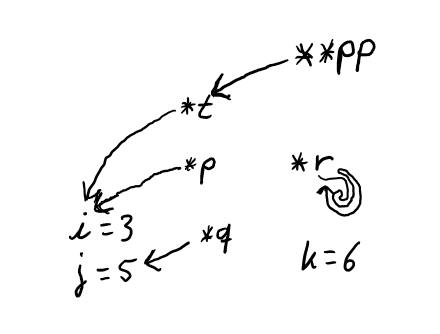
\includegraphics[width=300pt]{img/pointer.png}
\end{center}
\section*{2.b}
\begin{lstlisting}
wert = (p == i);
\end{lstlisting}
Wert ist = 0. Da bei p nicht der Wert, sondern die Adresse betrachtet wird sind nicht beide echt gleich.
\begin{lstlisting}
wert = *p / *q;
\end{lstlisting}
Hier wird 3/5 gerechnet und nur in ganzen Zahlen dargestellt, was hier 0 ist. Falls kein Leerzeichen zwischen / und *p steht denkt das Programm, es wird auskommentiert
\begin{lstlisting}
wert = *p / *q + 3;
\end{lstlisting}
Hier wird zu dem Ergebnis 3 von eben eine 3 hinzuaddiert, deshalb ist das Resultat 3.
\begin{lstlisting}
wert = **&p;
\end{lstlisting}
Wert ist = 3. Da der Wert hinter der Adresse auf die **p zeigt dargestellt wird.
\begin{lstlisting}
wert = *(r = &k);
\end{lstlisting}
Wert ist = 6. r wird auf die Adresse von k gesetzt und dann als Pointer zeigt r auf die Adresse von k mit dem Wert 6.
\begin{lstlisting}
wert = *(r = &k) = *p**q;
\end{lstlisting}
Wert ist = 15. Zuerst wird *r auf die Adresse von k gerichtet, dann wird die Adresse von k auf den Wert 15 (von 3(p)*5(q)) gesetzt und am Ende wir „wert“ diesem Wert gleichgesetzt.
\begin{lstlisting}
wert = *p***pp;
\end{lstlisting}
Wert ist = 9. Der Wert auf den p zeigt, wird mit dem Wert auf den q zeigt multipliziert und auf „wert“ gespeichert.



\chapter*{Aufgabe 2: Schach}

\textbf{(1) Aufbau eines Arrays, dass das Schachbrett und die Schachfiguren darstellen
kann}

Es wurde ein zweidimensionales char-Array (playground) initialisiert. Die Größe des Arrays ist über ein Makro (SIZE) definiert. In unserem Fall entspricht die Größe den Dimensionen eines Schachfeldes.
Bei dem Feld A1 fängt das Array bei [0][0] an. \\
Weiße Felder werden durch ein Leerzeichen dargestellt, für schwarze wird der Ascii-Code 177 verwendet.\\

\textbf{(2) String der Schachnotation in einzelne Züge aufschlüsseln}

Wurde mit \textbf{strtok} (string token) realisiert, durch Festlegen eines Trennzeichens (hier: „/“). Rückgabe ist ein Pointer, der auf die einzelnen gespaltenen Teile zeigt. In einer Schleife wird dieser Prozess wiederholt, bis alle Kommandos abgearbeitet wurden.\\

\textbf{(3) Automatisches Nachspielen der gegebenen Züge}

Nachdem ein Kommando aus dem Partie-String extrahiert wurde, wird die Funktion \textbf{play-str} aufgerufen und die Länge des Kommandos abgefragt. Bei einer Länge von 5 ist keine Spielfigur angegeben und es muss sich um einen Bauern handeln. Bei einer Länge von 6 ist die Spielfigur festgelegt.
Als nächstes wird überprüft, ob es sich um einen Setzzug oder Schlagzug handelt. Die Stelle des ausschlaggebenden Characters ist durch die bereits abgeschlossene Abfrage zur Länge des Kommandos eindeutig. \\
Durch die counter-Variable, die in jedem Schleifendurchlauf erhöht wird, kann überprüft werden, welcher Spieler gerade am Zug ist. Mit der Modulo-Operation wird überprüft, ob die Spielfigur als Groß- oder Kleinbuchstabe in das playground-Array gespeichert werden muss.
Anschließend wird die Funktion \textbf{update-playgroud} aufgerufen und das Spielfigur wird im Array auf die Zielposition gesetzt.
Das Startfeld wird entweder durch ein weißes oder schwarzes Feld ersetzt.\\

\textbf{(4) Darstellung des veränderten Schachbrettes auf dem Bildschirm}

Ausgegeben wird das Spielfeld mit einer einfachen for-Schleife in der Funktion \textbf{print-playground}.\\

\textbf{(5,6) Benutzer soll das Spiel weiterspielen}

Sobald der Partie-String vollständig gespielt wurde, wird in der main-Funktion gefragt ob der Spieler weiterspielen möchte oder nicht. Dies kann mit einer einfachen Eingabe von "j" bestätigt und mit "n" verneint werden. Falls die Frage mit einem "Nein" beantwortet wurde wird das Programm beendet. Falls weitergespielt werden möchte, wird die Funktion \textbf{play-input} aufgerufen.
Hier wird zunächst die Startposition und die Zielposition abgefragt. Bei der Eingabe von "00" als Startpostion wird das Spiel beendet.
Als nächstes werden die x- und y-Koordinaten der Startposition in Integer umgewandelt und die Figur, welche sich auf der Startposition befindet herausgearbeitet. Anschließend wird die Funktion \textbf{update-playground} aufgerufen und das Spielfeld wie bereits in (3) nachgespielt und anschließend auf der Konsole mit der Funktion \textbf{print-playground} ausgegeben.




% include sections like this


\end{document}
